\documentclass[letterpaper]{article}
\usepackage[top=1.0in,bottom=1.0in,left=1.0in,right=1.0in]{geometry}
\usepackage{verbatim}
\usepackage{amssymb}
\usepackage{graphicx}
\usepackage{svg}
\usepackage{longtable}
\usepackage{amsfonts}
\usepackage{amsmath}
\usepackage{hyperref}
\usepackage{float}
\usepackage{caption}
\usepackage{xcolor}
\def\thesection       {\arabic{section}}
\def\thesubsection     {\thesection.\alph{subsection}}

\author{Zoe Richter
        \\ \href{mailto:zrichte2@illinois.edu}{\texttt{zrichte2@illinois.edu}}
}

\title{Reactor Design Compilation}
\begin{document}
%\clearpage
\begin{titlepage}
\maketitle
\thispagestyle{empty}
\end{titlepage}

\section{Introduction}
To begin, take note of \cite{macpherson_molten_1985} and \cite{rosenthal_molten-salt_1970}.  These articles are not specific designs, instead, they give a general history of US MSR technology up to approximately 1980.  \cite{macpherson_molten_1985}, in particular, is a personal account of the author's experience in the growing field, and offers interesting insight.

This report seeks to collect various MSR designs and reprocessing techniques, and from them, complie a general list of MSR features.  The intent is to capture the expected varieties of fluid-fueled MSRs such that models and simulations can accommodate a broad range of designs.  The features given in this review include characteristics such as:

\begin{itemize}
\item Single fluid or two fluid salt
\item Single or multi-region core
\item neutron energy spectrum
\item moderator type
\item salt type (relates to single or two-fluid)
\item Intensity of processing
\end{itemize}

The processing in an MSR can also vary.  After the general reactor designs have been compiled, processing options will be as well.

\section{Molten Salt Reactor Experiment (MSRE)}
This reactor is given as the first MSR design.  Technically, the Aircraft Reactor Experiment is its predecessor, however, given its unsuitability as a commercial reactor (and the focus of this report on such reactors) it is not included in detail here.  The MSRE has general characteristics, described thusly: \cite{robertson_msre_1965}
\\
Below, a test of including svg graphics nicely:
\begin{figure}
  \centering
  \includesvg[width=1.0\linewidth, svgpath = figures/]{msreproc}
  \caption{I tried so hard}
  \label{fig:trying}
  
\end{figure}

Below, a test using tikz:
\begin{figure}[H]
  \centering
  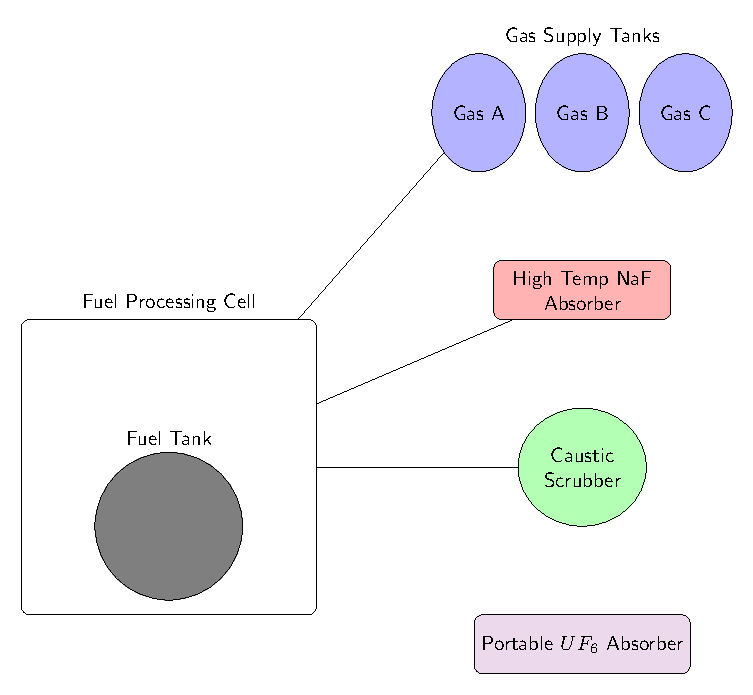
\includegraphics[width=1.0\linewidth]{figures/msretik.pdf}
  \captionof{figure}{And got so far}
  \label{fig:intheend}
\end{figure}


\begin{itemize}
\item 10 MW
\item Single-region
\item Graphite moderator
\item Fuel salt is a mix of lithium, beryllium, and zirconium fluoride salts, using either uranium or uranium and thorium.  Specifics of the composition are given in Table 2.1 of \cite{robertson_msre_1965}.
\item Total core volume is 90 cubic feet.  20 cubic feet is fuel, 70 cubic feet is graphite.
\item Graphite matrix is set in a rectangular grid, with 6 holes taken out to hold control rods.
\end{itemize}

\begin{figure}[H]
  \centering
  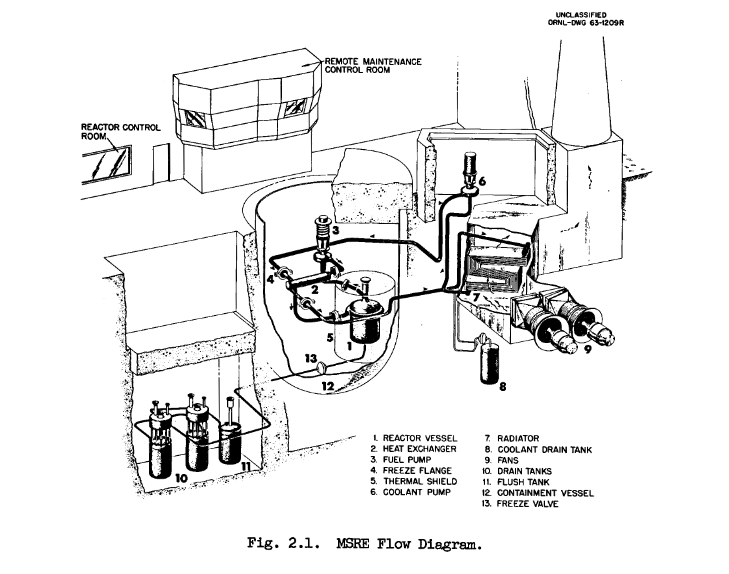
\includegraphics[width=1.0\linewidth]{figures/MSREsource1.png}
  \captionof{figure}{An image of the reactor building setup, from \cite{robertson_msre_1965} directly}
  \label{fig:fig1}
\end{figure}

\begin{figure}[H]
  \centering
  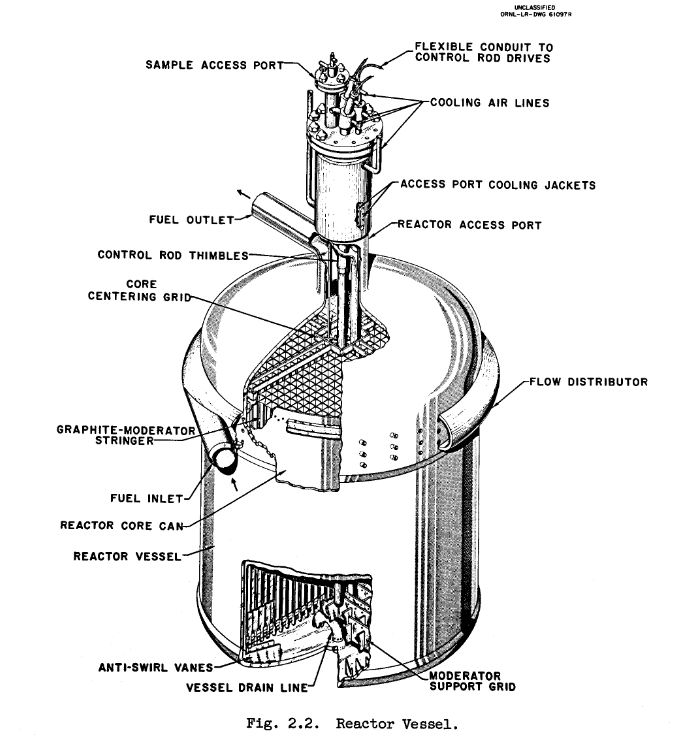
\includegraphics[width=1.0\linewidth]{figures/MSREsource2.png}
  \captionof{figure}{An image of the reactor core, from \cite{robertson_msre_1965} directly}
  \label{fig:fig2}
\end{figure}

There is not "online" reprocessing in this design, exactly.  When the fuel salts have become contaminated or otherwise undesireable, they are removed from the reactor, which is then flushed with a "flush salt".  This flush salt is simply the fuel salt mixture without any of the fissile isotopes added.

After chemical treatment, what can be saved from the salt is reused, the rest is disposed of.

\section{Molten Salt Breeder Reactor (MSBR)}
The MSBR builds on the MSRE, adding a conversion ratio high enough to classify the MSBR as a true breeder reactor.  It features a higher power in its design specifications, at the cost of a low graphite lifetime.  Additionally, it has a lesser fuel vol\% than the MSRE, and two fewer control rods.

\begin{itemize}
\item 1000 MWe, with a thermal plant efficiency of 44\%
\item Average core power density ~22kW/liter, with a plant factor of 80\%.  This gives:
	\begin{itemize}
	\item A four year graphite lifetime
	\item A fuel yield of 3.3\%
	\item A compounded fuel doubling time of 21 yr
	\end{itemize}
\item Reactor vessel is approximately 22ft in diameter and 20 ft high.
\item Core is 14.3ft in diameter and 13ft high
\item Salt to graphite ratio in the core is 13\%
\item Graphite moderator
\item Fuel salt is $LiF - BeF_2 - ThF_4 - UF_4$, using ${}^{233}U$ as the fissile isotope.  The concentrations in mole\%, from table 1 of \cite{bettis_design_1970}, is given as $71.6 - 16.0 - 12.0 - 0.4$, respectively.
\item Graphite matrix is a rectangluar grid with 4 control rod slots in the center.
\end{itemize}

\begin{figure}[H]
  \centering
  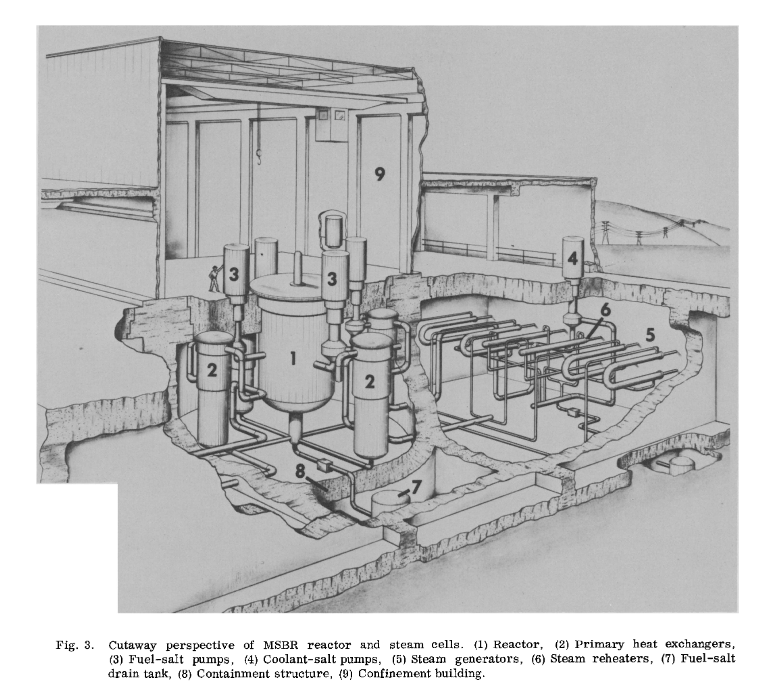
\includegraphics[width=1.0\linewidth]{figures/MSBRsource1.png}
  \captionof{figure}{An image of the reactor and steam systems, from \cite{bettis_design_1970}}
  \label{fig:fig3}
\end{figure}

\begin{figure}[H]
  \centering
  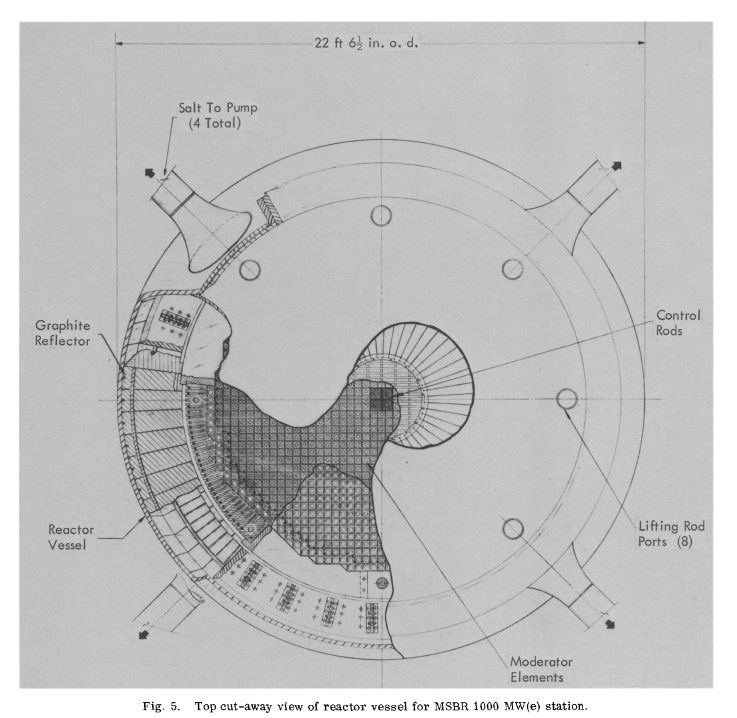
\includegraphics[width=1.0\linewidth]{figures/MSBRsource2.png}
  \captionof{figure}{A bird's eye view of the reactor core, from \cite{bettis_design_1970} }
  \label{fig:fig4}
\end{figure}

The chemical processing is more involved than the MSRE, and includes:
\begin{itemize}
\item An off-gas system to remove gaseous fission products, using helium spargers.
\item A continuous chemical processing loop to:
	\begin{itemize}
	\item Remove fission products
	\item Recover bred ${}^{233}U$
	\item Add more fertile material, as needed.
	\end{itemize}
\end{itemize}

\section{Molten Salt Demonstration Reactor (MSDR)}
A reactor concept from ORNL, hoping to build on the MSRE and show the commercial capabilities of an MSR.  The intention is to show the feasibility of a breeder MSR, however, the MSDR's conversion ratio isn't high enough to technically be a breeder.  Instead, it is a converter \cite{bettis_design_1972}.  One difference of note between the MSDR and the MSBR is that the  MSDR maintains a low enough power density that the graphite moderator is expected to last 30 years.  This is in stark contrast to the MSBR, which operates at a higher power density, and only anticipates a 4 year graphite lifetime.

\begin{itemize}
\item 350 MWe
\item Peak power density 114 W/cc
\item Reactor vessel is 26ft tall and 26ft in diameter
\item Graphite is used as the reflector in a square matrix, with graphite taking up 10\% of core volume
\item FLiBe salt, initially using ${}^{235}U$, that uses thorium to breed ${}^{233}U$
\item solid graphite slabs for reflector, arranged in an axial/ radial matrix.  Six slots in the matrix for control rods.
\end{itemize}

\begin{figure}[H]
  \centering
  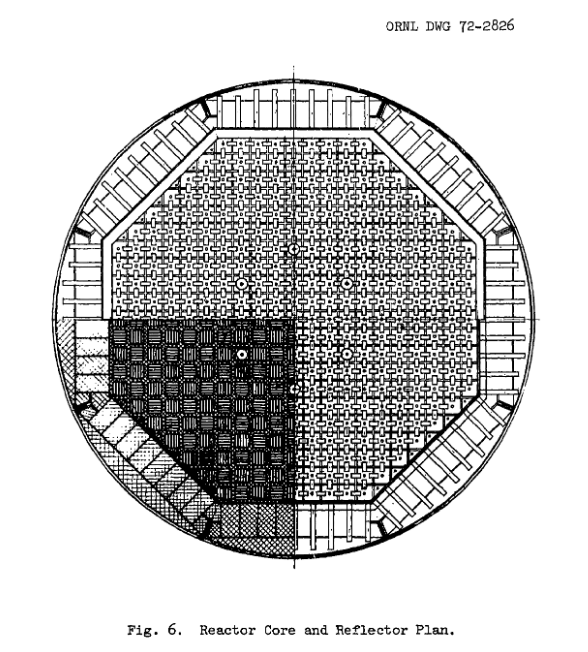
\includegraphics[width=1.0\linewidth]{figures/MSDRsource1.png}
  \captionof{figure}{The layout of the reactor core, from \cite{bettis_design_1972} }
  \label{fig:fig5}
\end{figure}

\begin{figure}[H]
  \centering
  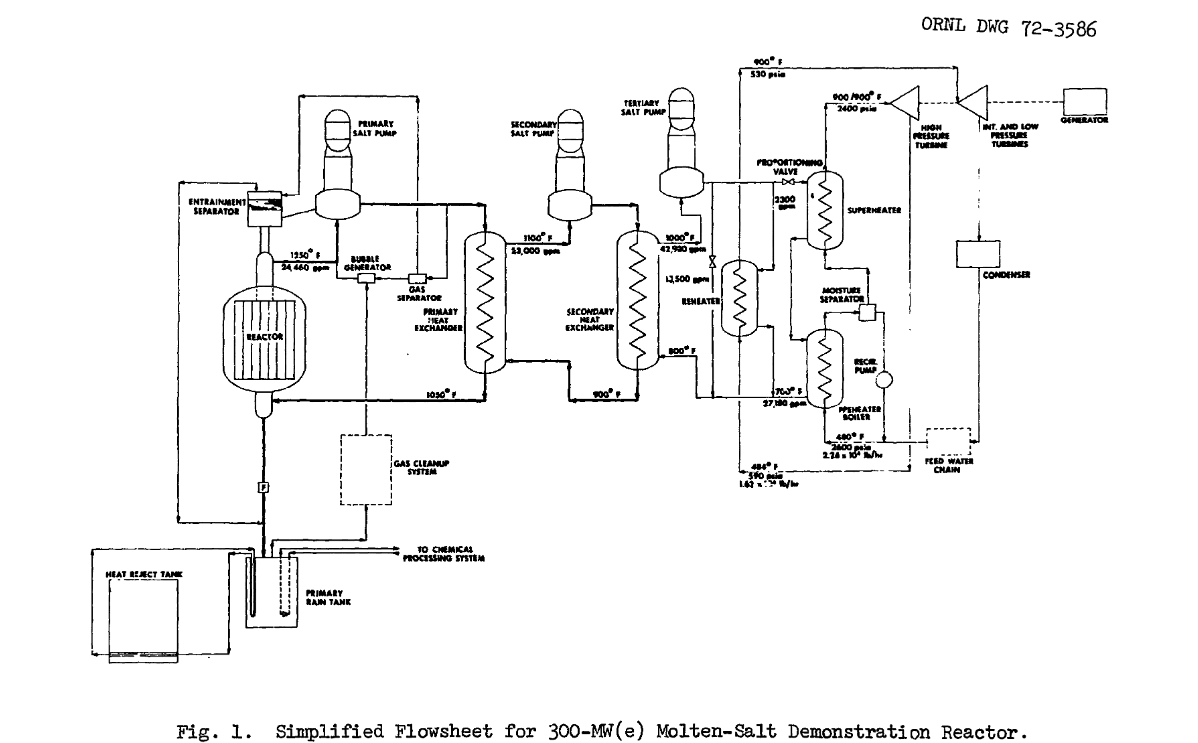
\includegraphics[width=1.0\linewidth]{figures/MSDRsource2.png}
  \captionof{figure}{Layout of the reactor, steam generation, and (most) of the salt processing, from \cite{bettis_design_1972} }
  \label{fig:fig6}
\end{figure}

The processing used in this reactor is minimal, and is intentionally limited to what was used in the MSRE.  All salt processing is as follows:

\begin{itemize}
\item A Hitec salt loop oxidizes tritium in the fuel salt into tritiated water for removal
	\begin{itemize}
	\item This salt loop goes to the heat exchanger for steam generation
	\end{itemize}
\item Xenon and other noble gases are removed via helium sparging
	\begin{enumerate}
	\item Initially, this gas spends 6 hrs in a drain tank
	\item Then, it is filtered for solids
	\item Approximately half of the filtered gas returns to the helium bubble generator, the other half spends 90 days in a charcoal clean-up system
	\end{enumerate}
\item Other fission products are not removed from the salt in a short time scale.  Instead, the salt is replaced every 8 years.  Fissile materials are taken from "spent" salt, where possible.
\end{itemize}

\section{Denatured Molten Salt Reactor (DMSR)}

This reactor is heavily based on the MSBR.  In fact, the design is mostly identical, except the DMSR does not remove fission products during the 30 year lifetime of design.  It does however, include helium sparging and some limited chemical processing to maintain salt quality.  This particular design is prompted by guidance given in 1976 by what is now the DOE, along with reports that concluded a breeder reactor without denatured fuel would not be able to be deployed worldwide, due to insufficient proliferation resistance. \cite{engel_conceptual_1980}

The basic qualities of this reactor are as follows:

\begin{itemize}
\item 1000 MWe power generation, with a low enough power density to give the graphite moderator a 30 year lifetime.
	\begin{itemize}
	\item Low power density also reduces neutron capture in ${}^{233}Pa$, to bolster nonproliferation
	\end{itemize}
\item Uses 20\% enriched ${}^{235}U$ to reach initial criticality.
\item Like the MSBR, uses $LiF - BeF_2 - ThF_4 - UF_4$ salt (with the above change in fissile isotope)
\item This reactor vessel is 10m in both height diameter, with the following core specifications:
	\begin{itemize}
	\item The core is 8.3m in height and diameter.
		\begin{itemize}
		\item The outer 95\% of the core volume, core B, has a salt volume of 12.94\%
		\item The inner 5\% of the core, core A, has a salt volume of 20\%
		\end{itemize}
	\end{itemize}
\item Table 9 and Table 10 in \cite{engel_conceptual_1980} give isotope concentrations and neutron utilization, as calculated for a few points in the reactor lifetime.
\end{itemize}

\begin{figure}[H]
  \centering
  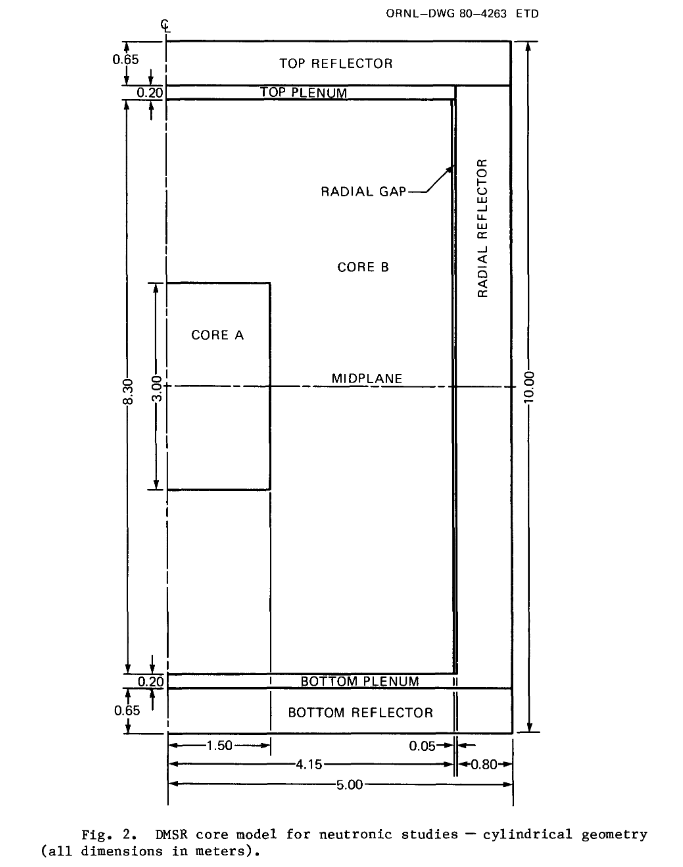
\includegraphics[width=1.0\linewidth]{figures/DMSRsource1.png}
  \captionof{figure}{A cut-away view of the core, from \cite{engel_conceptual_1980} }
  \label{fig:fig7}
\end{figure}

\section{Integral Molten Salt Reactor (IMSR)}

The IMSR400 is a small modular reactor (SMR) patented by Terrestrial Energy Inc.  The "core-unit" consists of the core, and integrated pumps and heat exchangers.  The core-unit has a lifetime of 7 years, but is made to be easily replaced, giving the designed plant an expected lifetime of 30 years.  Some specifics of this reactor, such as the fuel-coolant mixture, is proprietary, and explicit detail is not given.  What information is publicly available is as follows \cite{leblanc_18_2017}:

\begin{itemize}
\item 400 MWe, with an average core power density of 11-15 $\frac{MW}{m^{3}}$
\item Core is 4m in height, and 3.4m in diameter.
\item The length of each fuel cycle is 84 months, i.e., the 7-year lifetime of the core-unit
\item The moderator is graphite, and the shutdown rods are made of gadolinium oxide, and it does not have control rods
\item At the time of discharge, the average burnup is 26-29 MWd/kg
\item The salt mixture is a blend of fluoride salts, including sodium fluoride, berylium fluoride, and lithium fluoride.  At startup, the fuel has an enrichment of 2-3\%, and an enrichment of 5-19\% when used fissile material is replaced
\end{itemize}

\begin{figure}[H]
  \centering
  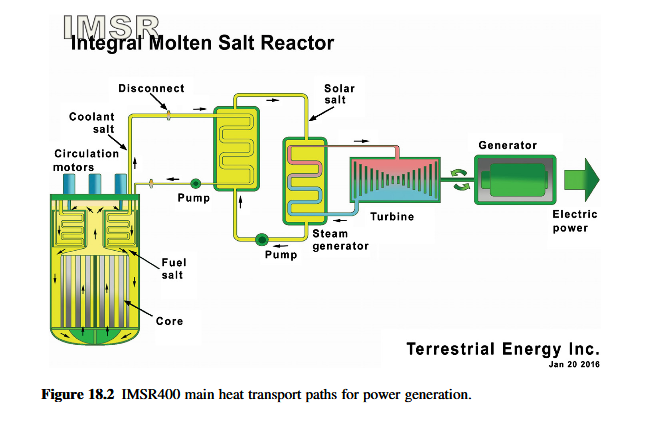
\includegraphics[width=1.0\linewidth]{figures/IMSRsource1.png}
  \captionof{figure}{A simplified view of the core-unit, and its attachment to the power generation loops, from \cite{leblanc_18_2017} }
  \label{fig:fig8}
\end{figure}

\begin{figure}[H]
  \centering
  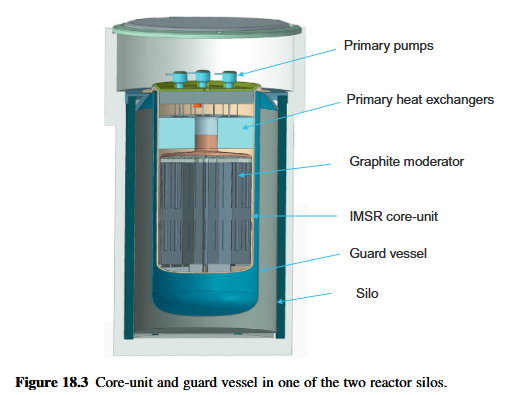
\includegraphics[width=1.0\linewidth]{figures/IMSRsource2.png}
  \captionof{figure}{The core, from \cite{leblanc_18_2017} }
  \label{fig:fig9}
\end{figure}

\section{Molten Salt Fast Reactor (MSFR)}
Of the reactors given in this review, this is one of the few fast reactors (the other being Terrapower's MCFR, given below).  Because such a reactor does not use a moderator, it circumvents some of the material contraints associated with degradation of the graphite moderator.  It also has a much higher breeding ratio.  This report uses a conceptual reference reactor with these characteristics \cite{rouch_preliminary_2014}: 

\begin{itemize}
\item A power of 3000 MWth
\item Three loops: the fuel, intermediate, and power conversion loops
\item Within the fuel circuit, there is a total salt volume of 18 cubic meters
	\begin{itemize}
	\item The fuel salt is lithium fluoride and actinide fluoride, with the mol\% of the actinide fluorides is assumed to be a fixed 22.5 mol\%
	\end{itemize}
\item Within the core, there is a fertile isotope blanket region, composed of a $LiF - ThF_4$ blend that has a concentration of $ThF_4$ of 22.5 mol\%
\item The blanket serves as the radial reflectors, to protect the reactor vessel.  On the top and bottom, there are reflectors made of nickel-based alloys.  This particular report also assumes this alloy will absorb 99\% of incoming neutrons.
\item The design initially used a very simple cylindrical geometry for the core, but by the time the report was written, the study moved on to more realistic, and complicated geometries.
	\begin{itemize}
	\item The first geometry is referred to as Geometry I.  The radial core walls are curved, along with the top reflector.  The bottom reflector is flat
	\item The second Geometry, Geometry II, features symmetrically curved walls within the core.  Both this and Geometry I are given in \ref{fig10} below.
	\end{itemize}
\item Helium sparging is assumed, but because its impact and the thermal-hydraulic properties was deemed neglible, it is neglected in calculations
\end{itemize} 

\begin{figure}[H]
  \centering
  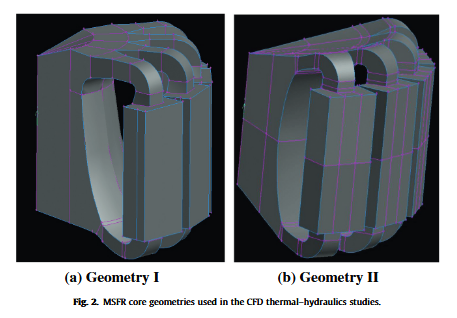
\includegraphics[width=1.0\linewidth]{figures/MSFRsource1.png}
  \captionof{figure}{Geometries I and II, from \cite{rouch_preliminary_2014}}
  \label{fig:fig10}
\end{figure}

In a separate report, \cite{doligez_coupled_2014} , a reactor with the same nominal power, and actinide mol\%.   While \cite{rouch_preliminary_2014} is focused on the thermal-hydraulic facets of an MSFR, \cite{doligez_coupled_2014} provides more in-depth information about the sort of fuel salt composition used in its reference model, and includes information on the reprocessing within the reference MSFR.

\begin{itemize}
\item This report gives the fissile salt explicitly: $LiF - ThF_4 - {}^{233}UF_4$ in with mol\% concentrations of $77.5\% - 20\% - 2.5\%$
\item The fertile blanket is 50 cm thick
\item The initial blanket salt is identical to the above report - $LiF - ThF_4$ in mol\% concentrations of $77.5\% - 22.5\%$

\end{itemize}

\section{Transatomic}

The Transatomic reactor has two important differences from other thermal-spectrum MSRs in this review.  It changes the fuel salt mixture, and forgoes a graphite moderator for something with a better lifespan under the conditions of the reactor \cite{robertson_assessment_2017}.

\begin{itemize}
\item The fuel salt is a $LiF - UF_4$ mixture, with a uranium concentration of 27.5\%
\item Unlike the other MSR designs reviewed, the Transatomic reactor uses a zirconium hydride moderator with corrosion resistant cladding
	\begin{itemize}
	\item Table 1 of \cite{robertson_assessment_2017} gives dimensional parameters for the moderator rods in the core
	\end{itemize}
\item Transtomic has proposed three fueling scenarios, but only the first has been the focus of ORNL studies:
	\begin{enumerate}
	\item 5\% start-up enrichment, followed by a 5\% online feed
	\item 5\% start-up enrichment, followed by an online feed of spent fuel from light water reactors
	\item 10\% start-up enrichment, followed by an online feed of 19.9\%
	\end{enumerate}
\item Burnup can be as high as 200 MWd/MTU, with the intention of limiting waste products
	\begin{itemize}
	\item After analysis of core models, with simulation of the chemical processing included with use of ChemTriton, the report concludes that after 15 years of operation, the reactor has bred enough plutonium to reach a burnup of 91.9 GWd/MTU by year 29.1 of operation
	\end{itemize}
\end{itemize}

\section{Terrapower}
website \href{https://terrapower.com/technologies/mcfr}{here}

Much of the current information about Terrapower's designs are in patents, and, therefore, not given in exact detail \cite{hyde_liquid_2015}.  However, it can be said that:

\begin{itemize}
\item The core has two regions, one fissile, one a fertile blanket.  The patent does not specify how exactly these regions are arranged, and also gives a homogenous mixture of the two materials as a possibility
\item ${}^{239}Pu$ is given as a possible isotope present in the fissile region, and ${}^{238}U$ as the fertile isotope in the fertile blanket
\end{itemize}

\bibliographystyle{plain}
\bibliography{2019-richter-msr-litrev}
\end{document}
